\subsection{Signal Model}

\begin{frame}[t]{Signal model}

    Sound propagation process $\Leftrightarrow$ Source $\to$ Filter $\to$ Receiver model

    \begin{equation*}
        \tikzmarknode{x}{}\contMic_i(t)
                = (
                    \textcolor{orange}{\contRIR_i}
                    \tikzmarknode{A}{\contConv}
                    \tikzmarknode{s}{\contSrc})(t) +
                    + \tikzmarknode{n}{\contNse(t)}
    \end{equation*}

    \begin{tikzpicture}[overlay,remember picture,
                        nodes={inner sep=1pt, align=center, font=\footnotesize},
                        gray,>=stealth] %
        \draw[->] (x.right) -- ++ (-8mm,+0mm) node[left] {{microphone signal}};
        \draw[->] (s.north) -- ++ (+12mm,+4mm) node[right] {{source signal}};
        \draw[->] (n.right) -- ++ (+8mm,+0mm) node[right] {{noise term}};
        \draw[->] (A.south) -- ++ (-4mm,-4mm) node[right] {{continuous-time convolution}};
    \end{tikzpicture}

    \vspace{-3mm}
    \hfill\textcolor{myred}{\small\faExclamationTriangle~ continuous time}

    % $\contMic_i$, $i$-th microphone signal $\contSrc$ source, signal $\contRIR_i$, $i$-th Room Impulse Response $\contConv$, continuous convolution

    % \vspace{5mm}
    % \begin{columns}[T,onlytextwidth]
    %     \begin{column}{0.48\textwidth}
    %         \centering
    %         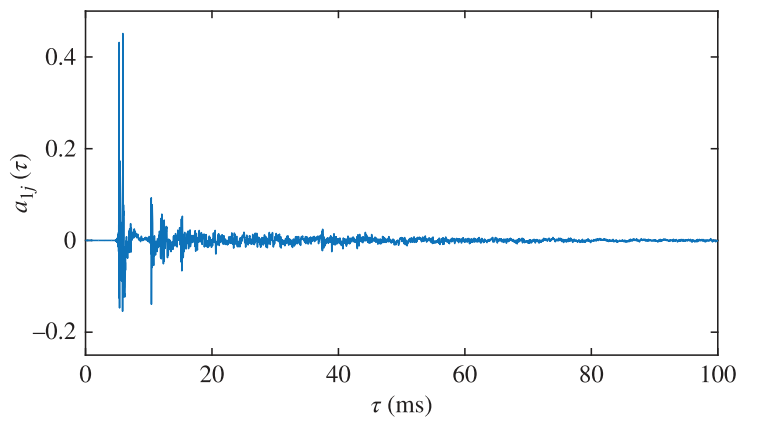
\includegraphics[width=\textwidth]{figures/rir_measured.png}
    %     \end{column}
    %     \begin{column}{0.48\textwidth}
    %         \centering
    %         \includegraphics<2>[width=\textwidth]{figures/rir_bang.png}
    %         \includegraphics<3->[width=\textwidth]{figures/rir_schematic.png}
    %     \end{column}
    % \end{columns}

    \begin{mydefblock}{Room Impulse Response (RIR)}
        \begin{itemize}
            \item linear filtering effect of the sound
            \item acoustic response of a room to a (prefect) impulsive sound
            \item depends on spatial properties (room geometry, mic/src position)
        \end{itemize}
    \end{mydefblock}

    \begin{columns}
        \column{0.48\textwidth}
            \centering
            % real RIR with part
            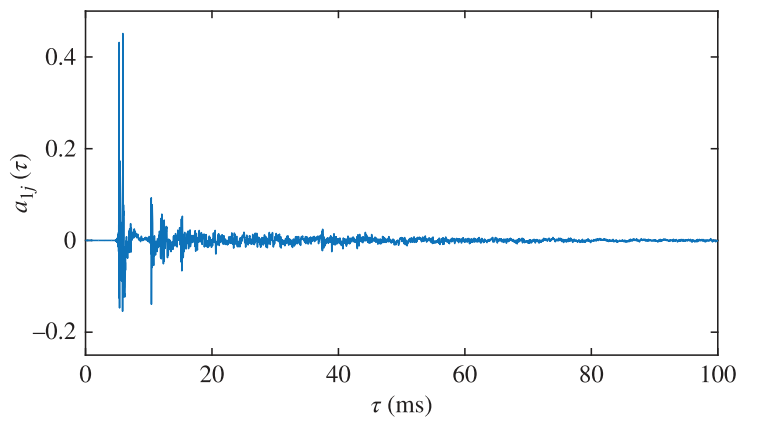
\includegraphics[width=0.8\textwidth]{figures/rir_measured.png}

        \column{0.48\textwidth}
            \centering
            % bang RIR
            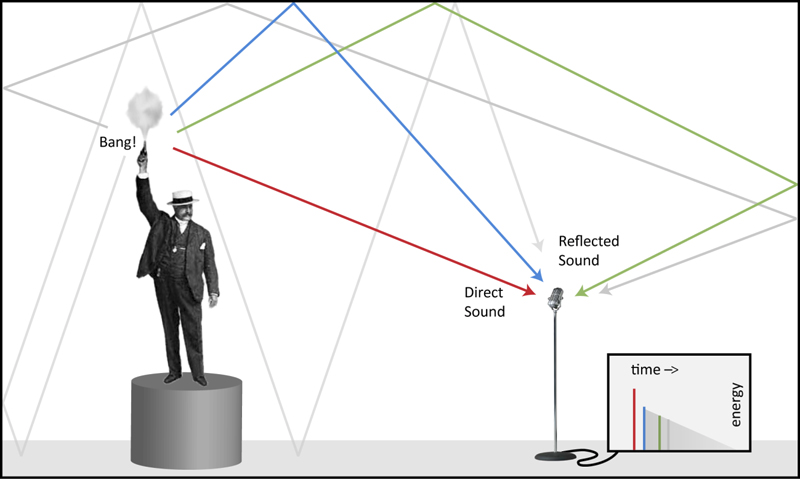
\includegraphics[width=0.8\textwidth]{figures/rir_bang.png}

    \end{columns}

\end{frame}


\subsection{Current Challenges}

\begin{frame}{Echoes in the RIR}

    RIR model
    \begin{columns}
        \column{0.48\textwidth}
        \begin{equation*}
            \contRIR_i(t) = \textcolor{myred}{\contRIRidirect}(t)
                          + \textcolor{myblue}{\contRIRiearly}(t)
                          + \textcolor{mygreen}{\contRIRilate}(t)
                          + \varepsilon_i(t)
        \end{equation*}

        \column{0.48\textwidth}
        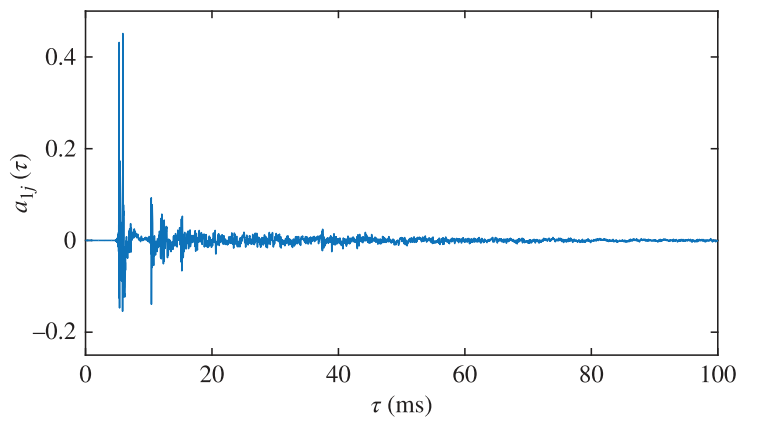
\includegraphics[width=.8\textwidth]{figures/rir_measured.png}

    \end{columns}

    Echoes can be modeled as sum of Dirac's delta

    \begin{equation*}
        \contRIR_i^\text{echoes} = \textcolor{myred}{\contRIRidirect}(t) + \textcolor{myblue}{\contRIRiearly}(t)
            \approx \sum_{r=0}^{R} \alpha_i^{(r)} \delta(t - \textcolor{orange}{\tau_i^{(r)}})
    \end{equation*}

    \textbf{Goal:} estimated the $\set{\tau_i}_{i,r}$

    \textbf{Challenges:}
    \begin{itemize}
        \item $\alpha$ distortion (even if we know it $\implies$ labeling)
        \item $\alpha \to \alpha(t)$ (sum of diracs $\to$ sum of filters)
        \item $h_l$ reverberation is included in the noise term
        \item depends on the scene geometry (room, source and mic position)
        \item presence of noise (interferences and measurements)
        \item sampling process (MULAN image)
    \end{itemize}

\end{frame}

% \begin{frame}{Echoes and Room Impulse Response}

%     \begin{columns}[onlytextwidth]
%         \begin{column}{0.60\textwidth}
%             \begin{block}{RIRs can be modeled with the Image Methods}
%                 \begin{itemize}
%                     \item \textbf{specular reflection} only
%                     \item for cuboid room, \textbf{it is} the sound prop.
%                     \item in general, \textbf{well models the early part} of RIRs.
%                     \item unique for each source and mic source
%                 \end{itemize}
%             \end{block}
%         \end{column}
%         \begin{column}{0.38\textwidth}
%             \centering
%             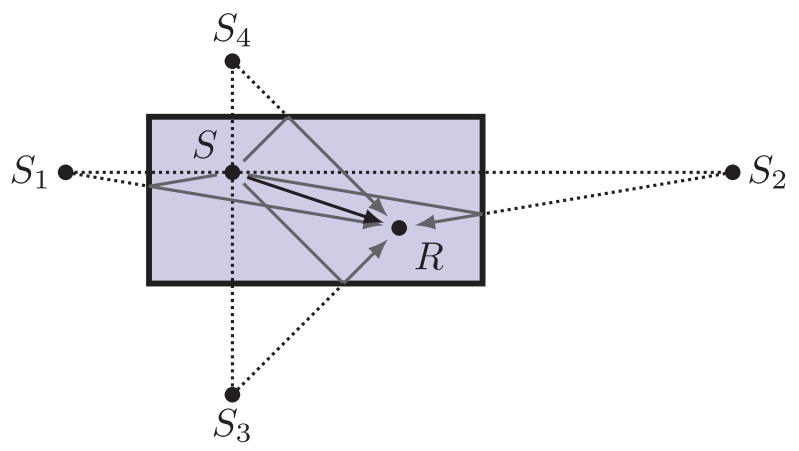
\includegraphics[width=0.8\textwidth]{figures/ism.png}
%             {\small\itshape ``playing billiard in a concert hall''}
%         \end{column}
%     \end{columns}

%     \vspace{2mm}
%     \pause
%     \begin{columns}[onlytextwidth]
%         \begin{column}{0.45\textwidth}
%             \centering
%             % \textbf{Time domain}
%             \begin{equation*}
%                 h_i^e(t) = \sum_{r=0}^{R} \alpha_i^{(r)} \delta(t - \tau_i^{(r)})
%             \end{equation*}
%             {\small sum of Dirac's delta}
%         \end{column}%
%         \pause
%         \begin{column}{0.05\textwidth}
%             \centering
%             $\overset{\text{more realistic}}{\longrightarrow}$
%         \end{column}%
%         \begin{column}{0.45\textwidth}
%             \centering
%             % \textbf{Frequency domain}
%             \begin{equation*}
%                 H_i^e(f) = \sum_{r=0}^{R} \alpha_i^{(r)}(f) \cste^{-\csti 2 \pi f \tau_i^{(r)}}
%             \end{equation*}
%             {\small sum of filters}
%         \end{column}
%     \end{columns}

%     \pause
%     \vfill
%     \begin{block}{RIRs accounts for}

%         \vspace{3mm}
%         \begin{columns}[T,onlytextwidth]
%             \column{0.48\textwidth}
%             the \textbf{geometry} of the room
%             \begin{itemize}
%                 \item \alert{Room shape and size}
%                 \item \alert{Mic and Source position}
%                 \item other objects (eg. reflectors)
%             \end{itemize}
%             \column{0.48\textwidth}
%             the \textbf{acoustic properties} of
%             \begin{itemize}
%                 \item surface materials
%                 \item objects materials
%             \end{itemize}
%         \end{columns}
%     \end{block}

%     \pause
%     \begin{mydefblock}{Echoes}
%         \centering
%         strong and distinct specular reflection
%     \end{mydefblock}

% \end{frame}

% \begin{frame}{Echoes in (Digital) Signal Processing}

%     \begin{block}{Room Impulse Response}
%         \begin{equation*}
%             \tilde{x}_i = (\tilde{h}_i \ast \tilde{s})(t) \longrightarrow \tilde{X}_i( f) = \tilde{H}_{ij}( f) \tilde{S}( f)
%         \end{equation*}
%         the linear filtering effect due to the propagation of sound from a source to a microphone in a indoor space
%     \end{block}

%     \begin{block}{Observation}
%         Our vision is limited both in time (finite and discrete) and in frequency (finite and discrete)
%         \begin{equation}
%             x_i[n] = ...
%         \end{equation}
%     \end{block}

%     \begin{block}{Signal model in the frequency domain}
%         \begin{equation*}
%             x_i = (h_i \ast s)(t)\;\longrightarrow\;X(f) = H_i(f) S(f)
%         \end{equation*}
%     \end{block}

%     \begin{block}{Approximations}
%         \begin{itemize}
%             \item Narrowband Approximation
%             \item DTFT echo model in the DFT
%         \end{itemize}
%     \end{block}

% \end{frame}

%% \subsection*{interim conclusion}
% \begin{frame}{Interim Conclusion I}
%     \begin{alertblock}{Approximations}
%         \begin{itemize}
%             \item Echoes are well described by specular reflection
%             \item Echoes are off-grid by nature
%             \item Sampling and quantization make them hard
%             \item Processing in the discrete frequency domain, but with continuous time echo model
%         \end{itemize}
%     \end{alertblock}
% \end{frame}
